\chapter{Deseño}

Neste capítulo explicaremos a arquitectura da plataforma empezando por unha visión xeral da mesma e despois comentando máis en detalle o deseño do servidor e da aplicación Android.


\section{Arquitectura xeral}

A nosa plataforma consta dos seguintes elementos (ver figura~\ref{fig:arq_xeral}):
\begin{itemize}
	\item Servidor base de datos (POIs e percorridos).
	\item Aplicación Android para visualización e edición de datos.
	\item Sistema de autenticación (GoogleAuth).
	\item Sistema de localización en interiores (Situm).
\end{itemize}


\begin{figure}[tb] 
	\begin{center}
		\includegraphics[width=0.65\textwidth]{figures/arqXeral}
		\caption{Arquitectura xeral da plataforma Caronte para a guía de museos.}
		\label{fig:arq_xeral}
	\end{center}
\end{figure}



%%%%%%%%
\section{Modelo de datos}
Neste punto exporase o modelo de datos da plataforma que se seguiu á hora da creación da base de datos. Na figura ~\ref{fig:modelo_datos} pódese observar o diagrama entidade relación. A continuación describirase cada táboa por separado:

\begin{figure}[tb] 
	\begin{center}
		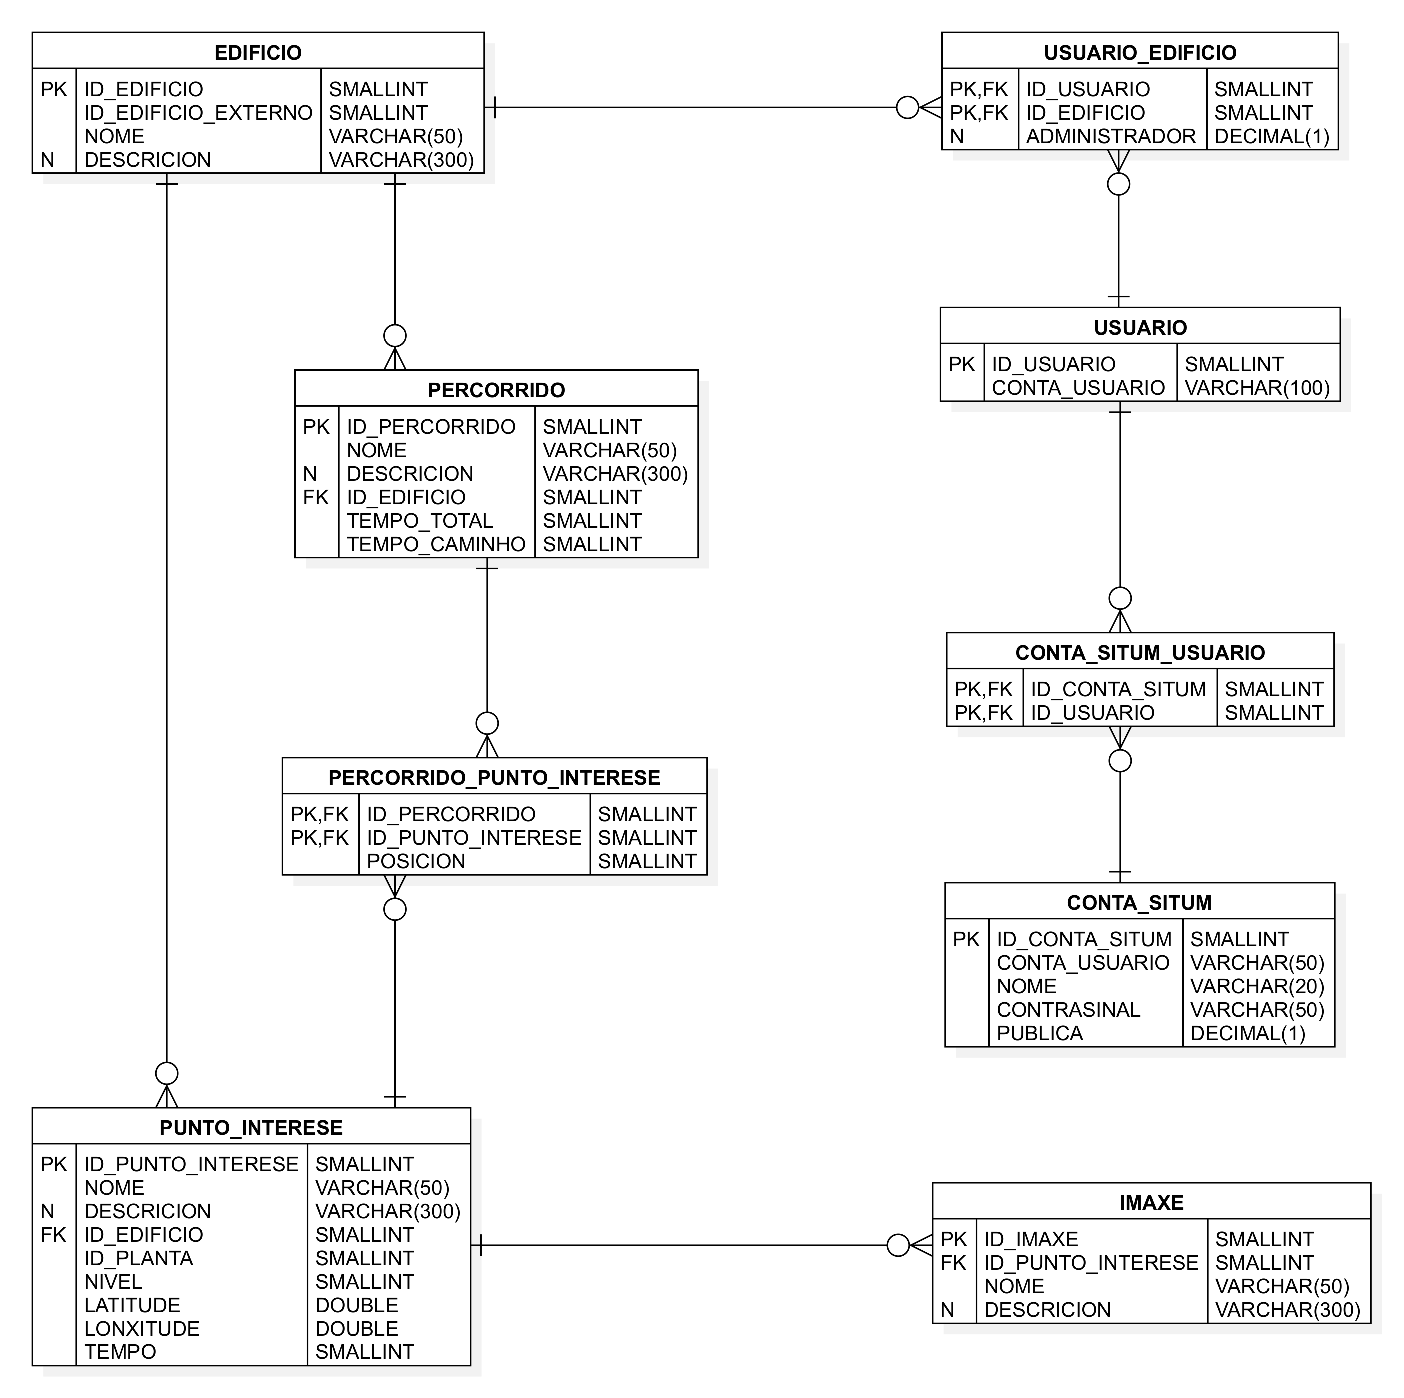
\includegraphics[width=0.95\textwidth]{figures/BD/diagramaEntidadeRelacion}
		\caption{Modelo de datos da plataforma Caronte.}
		\label{fig:modelo_datos}
	\end{center}
\end{figure}

\subsection{EDIFICIO}
Nesta entidade gardarase a información básica dos edificios que se tratan na aplicación. Aparte dos datos propios creados para a plataforma tamén se garda o identificador do edificio dentro do sistema Situm, que permite relacionar os edificios de Caronte cos de Situm.

As columnas das que se compón este entidade son:
\begin{itemize}
	\item ID\_EDIFICIO: Chave primaria autoxerada da táboa. De tipo SMALLINT (short). É o identificador do edificio dentro do sistema de Caronte. Non pode ter valor nulo.
	\item ID\_EDIFICIO\_EXTERNO: De tipo SMALLINT (short). É o identificador do edificio dentro do sistema de Situm.
	\item NOME: De tipo VARCHAR (string) con límite de 50 caracteres. É o texto que se visualizará na aplicación e que permite ao usuario a distinción entre edificios. Non pode ter valor nulo.
	\item DESCRICION: De tipo VARCHAR (string) con límite de 300 caracteres. Un breve texto explicativo sobre o edificio. Pode ter valor nulo.
\end{itemize}

\subsection{USUARIO}
Nesta entidade gardarase a conta de usuario coa que alguén se autentica na aplicación. Só se gardará o nome desa conta.

As columnas das que se compón este entidade son:
\begin{itemize}
	\item ID\_USUARIO: Chave primaria autoxerada da táboa. De tipo SMALLINT (short). É o identificador do usuario dentro do sistema de Caronte. Non pode ter valor nulo.
	\item CONTA\_USUARIO: De tipo VARCHAR (string) con límite de 100 caracteres. Correspóndese coa conta de correo de Google do usuario que se autentica na aplicación. Non pode ter valor nulo.
\end{itemize}

\subsection{USUARIO\_EDIFICIO}
Nesta entidade gardarase información sobre as accións que pode levar a cabo un usuario sobre un edificio concreto. A información desta entidade é a que indica se un usuario é un xestor de contido sobre un edificio.

As columnas das que se compón este entidade son:
\begin{itemize}
	\item ID\_USUARIO: Forma parte da chave primaria da entidade. Chave foránea da táboa USUARIO. De tipo SMALLINT (short). Non pode ter valor nulo.
	\item ID\_EDIFICIO: Forma parte da chave primaria da entidade. Chave foránea da táboa EDIFICIO. De tipo SMALLINT (short). Non pode ter valor nulo.
	\item ADMINISTRADOR: De tipo DECIMAL con límite 1 (boolean). Indica se o usuario é xestor de contido sobre o edificio.
\end{itemize}


\subsection{PUNTO\_INTERESE}
Nesta entidade gardarase información sobre os puntos de interese creados sobre un edificio e a súa localización exacta no planeta.

As columnas das que se compón este entidade son:
\begin{itemize}
	\item ID\_PUNTO\_INTERESE: Chave primaria autoxerada da táboa. De tipo SMALLINT (short). É o identificador do punto de interese. Non pode ter valor nulo.
	\item NOME: De tipo VARCHAR (string) con límite de 50 caracteres. É o texto que se visualizará na aplicación e que permite ao usuario a distinción entre puntos de interese. Non pode ter valor nulo.
	\item DESCRICION: De tipo VARCHAR (string) con límite de 300 caracteres. Un breve texto explicativo sobre o punto de interese. Pode ter valor nulo.
	\item ID\_EDIFICIO: Chave foránea da táboa EDIFICIO. De tipo SMALLINT (short). Permite identificar o edificio no que se atopa o punto. Non pode ter valor nulo.
	\item ID\_PLANTA: De tipo SMALLINT (short). É o identificador da planta dentro do sistema de Situm. Este dato permite maior rapidez á hora de identificador os puntos dunha planta. Non pode ter valor nulo.
	\item NIVEL: De tipo SMALLINT (short). Indica o número de planta no que se atopa un punto. Non pode ter valor nulo.
	\item LATITUDE: De tipo DOUBLE. Indica a latitude do punto, o que permite unha localización exacta nun mapa. Non pode ter valor nulo.
	\item LONXITUDE: De tipo DOUBLE. Indica a lonxitude do punto, o que permite unha localización exacta nun mapa. Non pode ter valor nulo.
	\item TEMPO: De tipo SMALLINT (short). Indica o tempo en minutos de media que lle leva a un visitante admirar unha obra. Non pode ter valor nulo e o seu valor por defecto é 0.
\end{itemize}


\subsection{PERCORRIDO}
Nesta entidade gardarase información sobre os percorridos dispoñíbeis nos edificios.

As columnas das que se compón este entidade son:
\begin{itemize}
	\item ID\_PERCORRIDO: Chave primaria autoxerada da táboa. De tipo SMALLINT (short). É o identificador do percorrido. Non pode ter valor nulo.
	\item NOME: De tipo VARCHAR (string) con límite de 50 caracteres. É o texto que se visualizará na aplicación e que permite ao usuario a distinción entre percorridos. Non pode ter valor nulo.
	\item DESCRICION: De tipo VARCHAR (string) con límite de 300 caracteres. Un breve texto explicativo sobre o percorrido. Pode ter valor nulo.
	\item ID\_EDIFICIO: Chave foránea da táboa EDIFICIO. De tipo SMALLINT (short). Permite identificar o edificio no que se atopa o percorrido. Non pode ter valor nulo.
	\item TEMPO\_TOTAL: De tipo SMALLINT (short). Indica o tempo en minutos de media que lle leva a un visitante realizar todo o percorrido contando co tempo que pase diante das obras. Non pode ter valor nulo e o seu valor por defecto é 0.
	\item TEMPO\_CAMINHO: De tipo SMALLINT (short). Indica o tempo en minutos de media que lle leva a un visitante realizar todo o percorrido sen contar o tempo que pase diante das obras. Non pode ter valor nulo e o seu valor por defecto é 0.
\end{itemize}


\subsection{PERCORRIDO\_PUNTO\_INTERESE}
Nesta entidade gardarase información sobre os percorridos dispoñíbeis nos edificios.

As columnas das que se compón este entidade son:
\begin{itemize}
	\item ID\_PERCORRIDO: Forma parte da chave primaria da entidade. Chave foránea da táboa PERCORRIDO. De tipo SMALLINT (short). Non pode ter valor nulo.
	\item ID\_PUNTO\_INTERESE: Forma parte da chave primaria da entidade. Chave foránea da táboa PUNTO\_INTERESE. De tipo SMALLINT (short). Non pode ter valor nulo.
	\item POSICION: De tipo SMALLINT (short). Indica a posición ordenada dun punto de interese dentro dun percorrido. Non pode ter valor nulo.
\end{itemize}


\subsection{CONTA\_SITUM}
Nesta entidade almacénanse as distintas contas de usuario dispoñíbeis na aplicación para o acceso á plataforma de Situm. Con elas permítese o tratamento de distintos edificios.

As columnas das que se compón este entidade son:
\begin{itemize}
	\item ID\_CONTA\_SITUM: Chave primaria autoxerada da táboa. De tipo SMALLINT (short). É o identificador da conta de Situm. Non pode ter valor nulo.
	\item CONTA\_USUARIO: De tipo VARCHAR (string) con límite de 50 caracteres. É o correo electrónico que utiliza Situm para autenticarse. Non pode ter valor nulo.
	\item NOME: De tipo VARCHAR (string) con límite de 20 caracteres. É o texto que se visualizará na aplicación e que permite ao usuario a distinción entre contas de Situm. Non pode ter valor nulo.
	\item CONTRASINAL: De tipo VARCHAR (string) con límite de 50 caracteres. É o contrasinal que permite a conexión ao sistema de Situm. Non pode ter valor nulo.
	\item PUBLICA: De tipo DECIMAL con límite 1 (boolean). Indica se a conta de Situm pode ser por calquera usuario ou en cambio debe ter permisos sobre ela. Non pode ter valor nulo.
\end{itemize}


\subsection{CONTA\_SITUM\_USUARIO}
Nesta entidade almacénanse as relacións entre os usuarios e as distintas contas de acceso a Situm sobre as que teñen permiso. Non almacena máis que esa relación.

As columnas das que se compón este entidade son:
\begin{itemize}
	\item ID\_CONTA\_SITUM: Forma parte da chave primaria da entidade. Chave foránea da táboa CONTA\_SITUM. De tipo SMALLINT (short). Non pode ter valor nulo.
	\item ID\_USUARIO: Forma parte da chave primaria da entidade. Chave foránea da táboa USUARIO. De tipo SMALLINT (short). Non pode ter valor nulo.
\end{itemize}


\subsection{IMAXE}
Nesta entidade almacénase a información sobre todas as imaxes subidas. Cada rexistro debe facer referencia a un punto de interese concreto.

As columnas das que se compón este entidade son:
\begin{itemize}
	\item ID\_IMAXE: Chave primaria autoxerada da táboa. De tipo SMALLINT (short). É o identificador da imaxe. Non pode ter valor nulo.
	\item ID\_PUNTO\_INTERESE: Chave foránea da táboa PUNTO\_INTERESE. De tipo SMALLINT (short). Permite identificar o punto de interese ao que fai referencia a imaxe. Non pode ter valor nulo.
	\item NOME: De tipo VARCHAR (string) con límite de 50 caracteres. É o texto que se visualizará na aplicación e que permite ao usuario a distinción entre imaxes. Non pode ter valor nulo.
	\item DESCRICION: De tipo VARCHAR (string) con límite de 300 caracteres. Un breve texto explicativo sobre a imaxe. Pode ter valor nulo.
\end{itemize}

%%%%%%%%
\section{Servidor}

Capas:
\begin{itemize}
	\item DAO: Capa de acceso a datos
	\item Manager: Xestión dos datos. Transaccionalidade.
	\item Controladores: Reciben as peticións.
\end{itemize}




%%%%%%%%
\section{API rest}

/sw/museo/edificios
Recupera todos os edificios dispoñíbeis na plataforma.
GET


/pois/{idEdificioExterno}
Recupera todos os POIs a partir do identificador dun edificio. O identificador é o de Situm
GET


/contas
Recupera todas as contas de Situm públicas, é dicir, as dispoñíbeis para os usuarios anónimos.
GET


/contas/{idUsuario}
Recupera as contas de Situm dispoñíbeis para un usuario, tanto as públicas como as privadas.
GET


/percorridos/{idEdificio}
Recupera os percorridos dun edificio.
GET


/percorridosidexterno/{idEdificioExterno}
Recupera os percorridos dun edificio a partir do seu identificador de Situm.
GET


/ppi/{idPercorrido}
Recupera os POIs (coas súas posicións) dun percorrido a partir do seu identificador.
GET


/percorrido/gardar
Crea ou modifica un percorrido
POST - PUT?


/comprobarUsuarioGoogle
Comproba a validez da autenticación de Google dun usuario. Se é a primeira vez que se autentica, crea o usuario en BD. Devolve información.
POST - PUT?


/poi/gardar
Crea ou modifica un POI
POST - PUT?


/percorrido/eliminar
Elimina un percorrido
POST


/poi/eliminar
Elimina un POI
POST


/imaxe/recuperar/{listaIdImaxeCSV}
Recupera unha lista de imaxes. A entrada está separada por comas.
GET


/recuperar/{idEdificio}/{idPoi}/{idImaxe}




/subir/{idEdificio}/{idPoi}/{nome}/{descricion}



/actualizar/{idImaxe}/{nome}/{descricion}



/eliminar/{idImaxe}



%%%%%%%%
\section{Aplicación Android}


Poucas actividades. O peso recae sobre todo en MapaActivity onde se amosa o mapa. (fragmento)


InicioActivity: Actividade de inicio onde se permite a autenticación en Google e a selección da conta de Situm.

DetallePoiActivity, DetallePercorridoActivity amosan a informacion dun POI ou percorrido concreto, permitindo a súa edición se o usuario ten permiso.


Un diagrama coa navegación entre pantallas



No paquete servizo están as clases que realizan as chamadas tanto ao noso servidor como aos servidores de Situm (paquete interno chamado situm). Unha clase por cada chamada para non mesturar lóxica distinta.

A comunicación con Situm só se realiza dende a aplicación Android.

Escolleuse unha única aplicación tanto para a consulta como para a edición para aproveitar a potencia que nos dá o mapa de interiores á hora de localizar os puntos desexados e marcalos directamente.


Lista de permisos necesarios para a execución.

